\chapter{超對稱性為何可能重要}

\lectureoverview{真空漲落串連起本章的各個主題。邊界條件產生卡西米爾力，圈效應威脅希格斯質量，新的虛粒子會改變規範耦合的跑動，而真空能則支配宇宙膨脹。這些問題促使人們考慮低能超對稱性，藉此穩定希格斯標度、提供暗物質候選者，並改善規範耦合的統一。接著，我們以格拉斯曼座標構造超場，並利用貝雷津積分抽取超對稱作用量。}

\section{反射板之間的真空漲落}

我們回到超對稱性，先釐清一個關於卡西米爾效應的問題。將兩塊平行的反射板相隔\(d\)放置。即使沒有任何實粒子，量子場仍有真空漲落。我們可以將它們想像成虛過程，或等價地，視為場的各振子模態的零點運動。板施加了邊界條件，因此板間允許的漲落不同於不受限制空間中的漲落。

重要的不是能量的絕對零點，而是間距改變時所產生的變化。以\(\mathcal E(d)=E(d)/A\)表示單位面積的真空能。一旦\(\mathcal E\)依賴於\(d\)，它便是位能，而單位面積所受的力為
\begin{equation}
\frac{F}{A}=-\frac{d\mathcal E}{dd}.
\end{equation}
因此，虛過程的重新排列會形成可觀測的力。以理想導體板為例，在熟悉的電磁學情況下，能量和壓力為
\begin{align}
\mathcal E(d)&=-\frac{\pi^2}{720\,d^3},\\
\frac{F}{A}&=-\frac{\pi^2}{240\,d^4},
\end{align}
單位為\(\hbar=c=1\)。\editorialnote{這些係數，以及能量每單位面積的\(d^{-3}\)與壓力的\(d^{-4}\)之間的區別，釐清了黑板上提出的量綱問題。這些是理想平行板的標準結果，並非本文在此推導所得。}負號表示吸引力。

\begin{classroomqa}
\audiencequestion{四次方描述的是力還是能量？ \lecturetimestamp{00:04:39}}
\lecturerresponse{在四維時空中的平行板情況下，單位面積的能量按\(d^{-3}\)衰減；對\(d\)微分後，單位面積的力則按\(d^{-4}\)衰減。恢復\(\hbar\)和\(c\)後，量綱分析便可確定這些冪次。}
\end{classroomqa}

有時人們會把這項計算概括為：平行板中斷了虛光子圈。只要不把這種圖像理解得太字面，它便有所助益。精確的計算考察的是允許的場模態頻譜如何改變，或等價地，量子有效作用量如何改變。無論採用哪種說法，都會得到相同的、隨間距改變的能量。

\begin{classroomqa}
\audiencequestion{卡西米爾力可能是排斥力，而非吸引力嗎？ \lecturetimestamp{00:07:48}}
\lecturerresponse{可能。力的正負號並非普遍固定，而是取決於場、幾何形狀、材料和邊界條件。費米子圈效應的圈符號往往與玻色子圈效應相反，這促成了黑板上提出的猜想；然而，單憑費米子統計，並不能普遍推出每個卡西米爾力都必定是排斥力。\editorialnote{這項限定以一般性的陳述取代了課堂上刻意保留試探性的回答，以免造成錯誤的普遍印象。}}
\end{classroomqa}

\subsection{什麼可以作為真空能的證據？}

卡西米爾力已經測得，原子的可觀測量也會受到真空圈效應影響。然而，這兩項事實本身都不能證明絕對真空能會產生引力。卡西米爾實驗測量的是邊界造成的能量差；描述同一個力時，無須賦予無界的絕對零點能總和任何可操作的意義。

決定性的檢驗來自引力。能量就是引力荷。如果空間真空帶有均勻的能量密度，它就必須進入愛因斯坦方程，並影響宇宙膨脹。因此，宇宙加速膨脹便是真空樣成分直接的引力證據。

\begin{classroomqa}
\audiencequestion{為什麼通俗介紹會把真空能說成很神秘，彷彿物理學家不知道它是什麼？ \lecturetimestamp{00:08:19}}
\lecturerresponse{量子場論指出，每個場都有零點貢獻，因此真空能的可能性並不神秘。真正令人困惑的是其數值：為什麼它的引力效應遠小於根據已知量子場和高能截斷所作的估計？令人驚訝的是它幾乎不存在，而不是它本身存在。}
\end{classroomqa}

多年來，觀測上限小得驚人，人們很容易在心理上傾向於將宇宙學常數精確設為零，並尋找能強制相消的原理。然而，改進後的宇宙學觀測發現它有一個很小但非零的值。這項發現並未使真空能在概念上變得陌生，卻讓其受抑制的程度之高變得無法忽視。具體比較取決於所假設的紫外標度，但每一種自然的高能估計都需要巨大的相消。

\section{單一超荷對多粒子態的作用}

在列舉支持超對稱性的理由之前，我們應先釐清一個可能的悖論。玻色子可以任意大量地佔據同一個模態，而費米子模態的佔據數只能是零或一。如果某種對稱性能互換玻色子與費米子，它會不會把同一模態中的一千個玻色子變成一千個受泡利不相容原理禁止的費米子？

不會。費米子生成元一次只改變一個量子。在振子模型中，令\(a\)湮滅一個玻色子，並令\(c^\dagger\)產生其費米子夥伴。一個超荷可以表示為
\begin{equation}
Q=c^\dagger a.
\end{equation}
作用在含有\(n\)個玻色子且不含費米子的態上時，
\begin{equation}
Q\ket{n,0}
=\sqrt n\,\ket{n-1,1}.
\end{equation}
一個玻色子被移除，一個費米子則被加入。再以同一個荷作用一次，結果為零：
\begin{equation}
Q^2=(c^\dagger)^2a^2=0.
\end{equation}
這就是從費米子產生算符繼承而來的冪零性。

\begin{classroomqa}
\audiencequestion{如果許多玻色子佔據同一個態，為什麼超對稱變換不會在該態中產生許多費米子，進而違反泡利不相容原理？ \lecturetimestamp{00:12:05}}
\lecturerresponse{生成元不會取代整個佔據態，而是使態的費米子數改變一個單位。同一個費米子荷不能像普通轉動生成元那樣反覆作用，因為它的平方為零。另一個互補的荷可以反轉這次互換，而兩者的混合反對易子則閉合於時間平移。}
\end{classroomqa}

最後一句至關重要。簡寫\(Q^2=0\)適用於單一手徵分量，或適用於剛才寫出的簡單荷；這並不表示超荷的每一種乘積都為零。在四維超對稱中，
\begin{equation}
\{Q_\alpha,\bar Q_{\dot\beta}\}
=2\sigma^\mu_{\alpha\dot\beta}P_\mu,
\end{equation}
而
\begin{equation}
\{Q_\alpha,Q_\beta\}=0,
\qquad
\{\bar Q_{\dot\alpha},\bar Q_{\dot\beta}\}=0
\end{equation}
則適用於沒有中心荷的最小代數。\editorialnote{這種分量形式精確地說明了課堂上的簡寫：同一個\(Q\)反覆作用會得到零，而超荷與其共軛的反對易子則生成平移。}

\section{考慮低能超對稱性的三個理由}

\begin{classroomqa}
\audiencequestion{除了相消真空能之外，還有其他支持超對稱性的動機嗎？ \lecturetimestamp{00:15:06}}
\lecturerresponse{有三個密切相關的動機：控制希格斯自能、可能存在穩定的暗物質粒子，以及規範耦合在高能下更精確地會合。這些動機都不能證明自然界實現了超對稱性，但合在一起，使超對稱性成為值得認真檢驗的理論。}
\end{classroomqa}

「\emph{低能超對稱性}」是相對而言的說法。這不表示超伴粒子在日常尺度下很輕，而是表示它們的質量沒有遠高於電弱尺度和加速器尺度。如果超伴粒子的質量被推得任意高，這三項論證都會減弱。

\subsection{保護希格斯尺度}

標量質量對高能物理特別敏感。示意而言，玻色子圈圖會產生如下形式的修正
\begin{equation}
\delta m_H^2\big|_{\mathrm B}
\sim +\frac{\lambda}{16\pi^2}\Lambda^2,
\end{equation}
其中\(\Lambda\)表示有效理論適用的能標。費米子圈圖則帶有相反的符號，
\begin{equation}
\delta m_H^2\big|_{\mathrm F}
\sim -\frac{|y|^2}{8\pi^2}\Lambda^2.
\end{equation}
係數取決於相互作用和場的多重度，但超對稱性會將它們聯繫起來，使夥伴粒子之間的主導紫外敏感性相消。\editorialnote{這些示意性的圈圖公式呈現了定性自能論證背後的數學關係，並非完整的標準模型希格斯質量計算。}

這一點很重要，因為希格斯場的真空期望值決定了電弱尺度。規範玻色子和費米子的質量遵循例如下列關係：
\begin{equation}
m_W=\frac{gv}{2},
\qquad
m_f=\frac{y_fv}{\sqrt2}.
\end{equation}
如果希格斯部門自然地被推向極高尺度，除非以極高的精確度調整裸參數來抵消輻射修正，否則我們熟悉的低能粒子譜就會消失。

精確超對稱會使相消完全成立，但觀測到的玻色子與費米子質量不相等，已排除精確超對稱。在軟破缺的超對稱理論中，二次敏感性轉為依賴超伴粒子的質量劈裂，示意而言：
\begin{equation}
\delta m_H^2
\sim
\frac{g^2}{16\pi^2}
\left(m_{\mathrm{soft}}^2-m_{\mathrm{ordinary}}^2\right)
\ln\frac{\Lambda^2}{m_{\mathrm{soft}}^2}.
\end{equation}
只有當劈裂不太大時，這種相消才仍然有用。

\subsection{暗物質級聯的穩定終點}

將粒子譜分成普通粒子及其超伴粒子。費米子有玻色子夥伴，玻色子則有費米子夥伴。如果相互作用保有一種區分這兩類粒子的宇稱，那麼超伴粒子衰變後必須留下另一個超伴粒子：
\begin{equation}
\widetilde X
\longrightarrow X+\widetilde Y
\longrightarrow X+Y+\widetilde Z
\longrightarrow\cdots.
\end{equation}
級聯衰變無法除去最後一個超伴粒子，因此最終會停在最輕超對稱粒子（LSP）。

常用的對稱性是\(R\)宇稱，
\begin{equation}
R_p=(-1)^{3(B-L)+2s}.
\end{equation}
標準模型粒子的\(R_p=+1\)，而其超伴粒子的\(R_p=-1\)。如果\(R_p\)是精確的，每個相互作用都會包含偶數個超伴粒子，LSP也就穩定。\editorialnote{超對稱性本身並不保證LSP穩定。穩定性需要守恆的\(R\)宇稱，或具有相同結果的其他對稱性；若沒有這種對稱性，LSP便可能衰變。}

暗物質必須至少存活一個宇宙學時間尺度。它還必須以足夠弱的方式相互作用，才能反覆穿過可見星系盤，而不損失大量能量。帶電或強作用的粒子群會發生散射、耗散能量，並傾向於像普通物質一樣塌縮至同一個薄盤結構。觀測到的延展暈則指向中性、弱作用的成分。

這無法唯一確定LSP。依模型和對稱性破缺的形式而定，候選者可能是電弱規範費米子與希格斯微子的中性混合態，也可能是引力微子。帶電或帶色荷的候選者受到嚴格限制。超對稱性提供的不是必然的答案，而是一種自然的機制，能產生中性且長壽的終點粒子。

\section{跑動耦合與統一的線索}

第三個動機從電荷屏蔽談起。測得的耦合會隨能量尺度改變，因為虛粒子會修飾相互作用。以電磁作用為例，插入光子傳播子中的電子—正電子圈會在長距離下屏蔽電荷。在更短距離，或更高的動量轉移下，探針之間的極化雲較少，因此有效電荷較大。

寫成
\begin{equation}
\alpha_i=\frac{g_i^2}{4\pi}.
\end{equation}
在一圈近似下，逆耦合會隨能量的對數線性跑動：
\begin{equation}
\frac{d\alpha_i^{-1}}{d\ln\mu}
=-\frac{b_i}{2\pi}.
\end{equation}
因此
\begin{equation}
\alpha_i^{-1}(\mu)
=\alpha_i^{-1}(\mu_0)
-\frac{b_i}{2\pi}\ln\frac{\mu}{\mu_0}.
\end{equation}
\editorialnote{這個一圈方程精確表達了以對數能量為橫軸所畫出的近似直線。閾值效應和高圈修正會使這些線略微彎曲。}

在電弱尺度以上，三個基本規範耦合分別屬於
\begin{equation}
U(1)_Y,\qquad SU(2)_L,\qquad SU(3)_c.
\end{equation}
這三個規範群。低能時用來建立直觀圖像的電磁耦合，是電弱對稱性破缺後前兩個耦合的組合。對量子色動力學（QCD）而言，非阿貝爾規範場會造成反屏蔽：強耦合在短距離下減弱，這就是漸近自由。因此，\(\alpha_3^{-1}\)會隨\(\ln\mu\)增加，而其他逆耦合的斜率則不同。

標準模型的曲線似乎朝彼此靠近，但不會在同一點相交。超伴粒子會改變虛圈效應，因而改變係數\(b_i\)。採用傳統的大統一理論歸一化時，
\begin{align}
(b_1,b_2,b_3)_{\mathrm{SM}}
&=\left(\frac{41}{10},-\frac{19}{6},-7\right),\\
(b_1,b_2,b_3)_{\mathrm{MSSM}}
&=\left(\frac{33}{5},1,-3\right).
\end{align}
若超伴粒子閾值接近 TeV 尺度，外推的超對稱曲線會在
\begin{equation}
M_{\mathrm{GUT}}\sim 10^{16}\ \mathrm{GeV}.
\end{equation}
附近更精確地會合。沒有任何實驗能直接達到該尺度。我們測量低能耦合，由場的內容決定跑動，再將曲線外推許多個數量級。兩條線總會在某處相交；三條彼此獨立的線在同一點附近會合，才是非平凡的觀察。

\begin{classroomqa}
\audiencequestion{改進後的外推是否假設超對稱性精確成立，且超伴粒子質量彼此相等？ \lecturetimestamp{00:38:09}}
\lecturerresponse{不是。超對稱性已破缺，因此粒子質量有所劈裂。關鍵在於超伴粒子的圈效應何時開始影響跑動。如果超伴粒子不太重，斜率會提早改變，讓三個耦合趨於會合。如果它們重得驚人，超對稱閾值便太晚才出現，改進後的會合也就不復存在。}
\end{classroomqa}

閾值修正和未知的高能粒子譜，使我們不能照字面宣稱三條線在數學上精確相交。即便如此，結果仍然相當顯著：同一個有助於穩定希格斯尺度、並提供熱暗物質候選者的近似超伴粒子尺度，也改善了規範耦合的統一。

\subsection{引力與共同的高能尺度}

引力的表現不同，因為引力荷就是能量本身。在質心能量\(E\)下，一個有用的無量綱量度為
\begin{equation}
\alpha_G(E)\sim GE^2
=\left(\frac{E}{M_{\mathrm{Pl}}}\right)^2.
\end{equation}
在一般能量下，這個量小得驚人，但會隨\(E\)的平方增加。因此，它的倒數下降得遠比對數跑動的規範耦合逆值快，並在普朗克尺度附近達到約一的量級。

這項比較暗示，所有相互作用可能都受相近的高能尺度支配，但它不像規範耦合統一那樣明確。規範耦合是可重整場論中的無量綱參數；牛頓常數則有量綱，因此若要把引力放到同一張圖上比較，就必須另作約定。

\begin{classroomqa}
\audiencequestion{超伴粒子也參與相同的三種規範相互作用嗎？還是它們代表新的力？ \lecturetimestamp{00:42:35}}
\lecturerresponse{超伴粒子帶有與其夥伴相同的規範量子數。超電子帶有與電子相同的電荷；超夸克則帶有相應夸克的色荷和電弱荷，雖然兩者的自旋和質量不同。因此，超伴粒子的圈效應會修正相同的規範相互作用，而不會引進三種新的力。}
\end{classroomqa}

\begin{classroomqa}
\audiencequestion{如果在大型強子對撞機（LHC）發現一個超伴粒子，是否就能確證超對稱性？ \lecturetimestamp{00:43:27}}
\lecturerresponse{僅憑名稱，一個陌生粒子的發現還不足以證明什麼；但若發現的超伴粒子譜符合自旋、電荷、質量與耦合之間的超對稱關係，就會極具辨識性。超對稱性施加許多彼此關聯的限制，因此詳細的相互作用模式將提供決定性的檢驗。}
\end{classroomqa}

\subsection{尺度不能毫無代價地任意提高}

如果超伴粒子的質量只略高於實驗可及範圍，這三項動機仍都可能成立。如果其質量提高數個數量級，每項論證都會變弱：
\begin{enumerate}
\item 希格斯質量的相消會留下對質量劈裂仍高度敏感的殘餘效應。
\item 傳統的弱尺度熱遺跡不再以預期的尺度產生。
\item 規範耦合跑動的閾值移至更高處，三個耦合也就較不精確地會合。
\end{enumerate}
超對稱性仍可能存在於高得多的尺度，但它將無法再以同樣簡潔的方式解決這些特定的低能問題。某個想法流傳已久，並不代表自然界必定採用它；這只能說明該理論自洽，值得接受決定性的檢驗。

\section{宇宙學能告訴我們哪些暗物質資訊，又有哪些無法得知}

\begin{classroomqa}
\audiencequestion{標準宇宙學能否像核合成限制氫和氦的含量一樣，確定暗物質的總量和每個暗物質粒子的質量？ \lecturetimestamp{00:46:32}}
\lecturerresponse{宇宙學能相當精確地測出暗物質的總質量密度，但單靠密度無法區分粒子質量和數量。同樣的密度可能由少數重粒子構成，也可能由數量極多的極輕粒子構成。要辨認微觀粒子，還需要額外的理論或非引力觀測。}
\end{classroomqa}

兩種大致的可能性說明了這種模糊性。一種是接近電弱或 TeV 尺度的弱作用粒子，能從熱浴中凍結脫離熱平衡。另一個極端則是極輕的玻色子，例如軸子，能形成相干場組態或凝聚態。這兩種發展最充分的機制位於相反的尺度端點附近，並不表示中間的可能性就被排除。

暈的結構本身提供了一項重要限制。暗物質穿過普通物質時幾乎不受摩擦，因此能維持空間上的延展分布，而不會塌縮成發光物質的盤狀結構。旋轉曲線和其他引力現象告訴我們質量確實存在，但單憑這些現象無法得知粒子數量。

\begin{classroomqa}
\audiencequestion{早期宇宙是否可能起初只有超粒子，後來它們再衰變成我們觀測到的粒子？ \lecturetimestamp{00:49:11}}
\lecturerresponse{當溫度遠高於所有相關質量時，快速反應會使各種粒子趨向熱平衡，而不是維持任意的單邊分布。若超伴粒子數量不足，普通粒子的碰撞會產生超伴粒子；超伴粒子的碰撞和衰變則會補充普通粒子。精確的豐度取決於相互作用和自由度，但熱電漿會持續趨向平衡。}
\end{classroomqa}

宇宙冷卻時，有質量的粒子種類會受到波茲曼因子的抑制，並發生湮滅或衰變。當穩定的LSP之相互作用速率慢於宇宙膨脹率時，它便不再跟隨平衡態：
\begin{equation}
\Gamma_{\mathrm{ann}}
\sim n\langle\sigma v\rangle
\lesssim H.
\end{equation}
剩下的粒子形成遺跡豐度。\editorialnote{這個凍結條件以標準的定量判據補足了熱平衡的論述。其他LSP候選者，尤其是耦合極弱的引力微子，可能具有非熱的演化史。}

\begin{classroomqa}
\audiencequestion{LSP是什麼普通粒子的夥伴？它一定完全不與其他粒子相互作用嗎？ \lecturetimestamp{00:51:05}}
\lecturerresponse{這沒有與模型無關的答案。可行的暗物質LSP預期應為電中性且不帶色荷，但不必完全沒有相互作用。它可能是與光子、弱規範玻色子和希格斯場相關的混合態，也可能是引力微子。其確切身分取決於超對稱破缺後的粒子譜。}
\end{classroomqa}

\section{真空圖、自能圖與膨脹}

\begin{classroomqa}
\audiencequestion{希格斯發散和真空能發散有什麼不同？ \lecturetimestamp{00:52:09}}
\lecturerresponse{真空圖沒有外部粒子線；它會改變空間真空的有效作用量，並對真空能有所貢獻。希格斯自能圖有兩條外部希格斯線；它會改變希格斯傳播子，進而改變希格斯質量。兩者都涉及虛漲落，但所回答的是不同問題。}
\end{classroomqa}

我們可以把實粒子想像成插入真空中的雜質。與這個雜質相連的真空漲落會改變它的傳播和質量。卡西米爾板也會改變真空漲落，但原因是宏觀邊界條件。兩者共有的要素，是量子漲落會對置入其中的對象產生響應；不過，各情況下被修正的可觀測量並不相同。

\vspace{-2pt}
\subsection{物質、輻射與真空的稀釋方式各不相同}

令\(a(t)\)為宇宙標度因子，並令
\begin{equation}
H=\frac{\dot a}{a}
\end{equation}
表示哈伯參數。均勻宇宙中的局部應力能量守恆給出
\begin{equation}
\dot\rho+3H(\rho+p)=0.
\end{equation}
若狀態方程為\(p=w\rho\)，積分後可得
\begin{equation}
\rho(a)\propto a^{-3(1+w)}.
\end{equation}
\editorialnote{連續性方程簡潔地推導出粒子計數和波長拉伸這兩種說明背後的關係。}

對冷的非相對論性物質而言，\(p\approx0\)，因此
\begin{equation}
\rho_m\propto a^{-3}.
\end{equation}
固定的共動體積隨\(a^3\)增大，而其中粒子所帶的靜止能量大致不變。

對輻射而言，\(p=\rho/3\)，因此
\begin{equation}
\rho_r\propto a^{-4}.
\end{equation}
數密度的稀釋貢獻了三個冪次；第四個冪次則來自紅移：
\begin{equation}
\lambda\propto a,
\qquad
E_\gamma=\frac{2\pi\hbar c}{\lambda}\propto a^{-1}.
\end{equation}

\begin{classroomqa}
\audiencequestion{如果光子有波函數，推導稀釋定律時，為什麼可以把它當成粒子而非波來描述？ \lecturetimestamp{00:58:21}}
\lecturerresponse{這種區分不影響標度關係。以粒子描述時，共動體積內的粒子數固定，每個量子的能量都按\(a^{-1}\)紅移。以經典波描述時，波長會拉長，場能量也以相同的幅度下降。哪種說法較容易看出膨脹的影響，就可以採用哪種。}
\end{classroomqa}

真空能的狀態方程為\(p_\Lambda=-\rho_\Lambda\)，因此
\begin{equation}
\rho_\Lambda=\text{constant}.
\end{equation}
它不會隨空間膨脹而稀釋。事實上，一個共動區域包含的真空能為
\begin{equation}
E_\Lambda=\rho_\Lambda a^3V_0,
\end{equation}
會隨其物理體積增大。這便引出我們稍後將討論的能量守恆問題。

不同的冪次描繪出宇宙的演化：輻射下降最快，物質下降較慢，真空能則完全不下降。因此，微小的真空能項在早期宇宙可以忽略，到了晚期卻可能占據主導。依據此處討論的粗略數值，目前的能量組成約有\(70\%\)是真空能、\(30\%\)是物質，輻射所占比例則小得多。

\section{幾何等於能量}

愛因斯坦方程的時間—時間分量，將前述標度律轉化為動力學。黑板上的內容從一句口號和一個幾何項開始。

\begin{figure}[H]
\centering
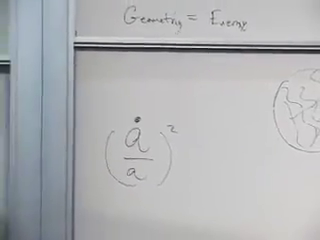
\includegraphics[width=0.68\textwidth]{lecture_06_figure_03.png}
\lectureframe{01:06:37.088}
\caption{黑板上的核心口號是\emph{幾何等於能量}，下方寫著膨脹項\(H^2=(\dot a/a)^2\)。}
\end{figure}

對均勻且各向同性的宇宙，第一條弗里德曼方程為
\begin{equation}
H^2+\frac{k}{a^2}
=\frac{8\pi G}{3}\rho,
\end{equation}
採用\(c=1\)的單位制，其中\(k=+1,0,-1\)表示空間幾何為閉合、平坦或開放，而
\begin{equation}
\rho
=\rho_{\mathrm{ordinary}}
+\rho_{\mathrm{dark}}
+\rho_{\mathrm{radiation}}
+\rho_{\mathrm{vacuum}}.
\end{equation}
\(1/a^2\)旁的正負號，取決於曲率項是留在等式左側，還是移到右側，也取決於\(k\)的取值。

\begin{figure}[H]
\centering
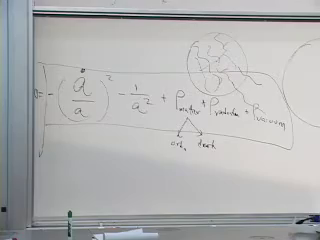
\includegraphics[width=0.96\textwidth]{lecture_06_figure_04.png}
\lectureframe{01:08:46.794}
\caption{完整的黑板平衡式：幾何側包含膨脹和空間曲率，來源側則包含物質、輻射和真空能。物質又分為普通物質與暗物質。}
\end{figure}

\subsection{宇宙學哈密頓約束}

\begin{classroomqa}
\audiencequestion{如果共動區域中的真空能隨宇宙膨脹而增加，那麼是否存在恆定的淨能量密度，或守恆的總能量？ \lecturetimestamp{01:01:51}}
\lecturerresponse{廣義相對論並未為任意膨脹時空提供普遍的全域能量。然而，在均勻宇宙學的約化描述中，愛因斯坦方程的時間—時間分量就是哈密頓約束。將幾何和物質放在同一側時，受約束的哈密頓量為零。變化的物質項由引力自由度來平衡，而非由盒子中某個一般意義上的固定能量來平衡。}
\end{classroomqa}

概略地說，標準表述為
\begin{equation}
\mathcal H_{\mathrm{gravity}}
+\mathcal H_{\mathrm{matter}}
=0.
\end{equation}
「總能量為零」這句話的確切含義就是如此。這是時間重參數化不變性所要求的運動方程，並非聲稱每個局域能量密度都為零。在共動體積中，普通物質的能量大致維持不變，輻射能量則減少，真空能則增加；與此同時，引力貢獻與膨脹率會相應調整，使愛因斯坦約束式持續成立。

局域守恆仍然嚴格成立：
\begin{equation}
\nabla_\mu T^{\mu\nu}=0.
\end{equation}
對均勻流體而言，這正是連續性方程
\(\dot\rho+3H(\rho+p)=0\)。一般而言，失效的是平直時空的直覺：認為在膨脹宇宙中，必定還有一個與座標無關且守恆的物質能量全域總和。\editorialnote{這項區分讓課堂上「能量始終為零」的說法有了精確含義：局域協變守恆與宇宙學哈密頓約束式都嚴格成立，但一般而言，並沒有唯一且定義良好的物質加引力全域能量。}

\begin{classroomqa}
\audiencequestion{零約束式是決定宇宙屬於開放、閉合還是平坦的條件嗎？\lecturetimestamp{01:04:42}}
\lecturerresponse{不是。哈密頓約束式在所有情況下都成立。開放、平坦與閉合宇宙的差異，取決於曲率標記\(k\)，因此也反映在\(k/a^2\)項上。曲率會改變平衡中的一項貢獻，但不會使這項約束式失效或生效。}
\end{classroomqa}

\section{格拉斯曼座標與超場}

\begin{classroomqa}
\audiencequestion{格拉斯曼數真的會出現在理論的拉格朗日量中嗎？\lecturetimestamp{01:09:37}}
\lecturerresponse{它們首先會出現，是因為費米子場是格拉斯曼奇場；其次，它們也作為超空間的座標出現。超場依賴這些奇座標，而超對稱作用量則透過對這些座標求導與積分來構造。}
\end{classroomqa}

普通場是時空的函數，
\begin{equation}
\phi=\phi(x^\mu).
\end{equation}
在四維最小超對稱理論中，\(x^\mu\)會擴充為一個二分量奇旋量\(\theta^\alpha\)及其共軛\(\bar\theta^{\dot\alpha}\)：
\begin{equation}
z^M=(x^\mu,\theta^\alpha,\bar\theta^{\dot\alpha}).
\end{equation}
這裡有兩個複數奇分量，或等價地說，四個實奇方向。超場是定義在這個超空間上的函數：
\begin{equation}
\Phi=\Phi(x,\theta,\bar\theta).
\end{equation}

這些並非度規意義下的微小空間維度。格拉斯曼座標沒有正的數值大小。說它很小，只是幫助理解冪零性的一種說法：
\begin{equation}
(\theta^\alpha)^2=0,
\qquad
\theta^\alpha\theta^\beta=-\theta^\beta\theta^\alpha.
\end{equation}
展開之所以會在有限項後終止，是因為冪零性，而非數值上的微小。\editorialnote{}

有四個獨立奇座標時，一般超場至多包含\(2^4=16\)個格拉斯曼單項式。概略地說，
\begin{equation}
\begin{aligned}
\Phi(x,\Theta)={}&\phi(x)+\Theta_A\psi_A(x)\\
&+\frac{1}{2}\Theta_A\Theta_B Z_{AB}(x)+\cdots\\
&+\Theta_1\Theta_2\Theta_3\Theta_4D(x),
\end{aligned}
\end{equation}
其中\(\Theta_A\)統稱這四個實奇座標。由於整個超場可以取為偶的，偶次項的係數是玻色場，奇次項的係數是費米場。因此，一個超場便能收納由普通分量場組成的有限多重態。

這種收納不只是記號上的便利。超對稱在幾何上表現為奇方向上的平移與時空平移相互混合。依照超空間規則以超場構造的拉格朗日量，會繼承超對稱；這就如同以張量構造的標量拉格朗日量會繼承旋轉或洛倫茲不變性。

作用量現在包含格拉斯曼測度。典型的全超空間項形式如下：
\begin{equation}
S_D=\int d^4x\,d^2\theta\,d^2\bar\theta\,
\mathcal K(\Phi,\Phi^\dagger).
\end{equation}
手徵項則使用以下測度：
\begin{equation}
S_F=\int d^4x\,d^2\theta\,W(\Phi)+\mathrm{h.c.}
\end{equation}
\editorialnote{全超空間測度與手徵測度的區分，是對示意性的\(d^4x\,d^4\theta\)作用量所作的標準細化。要採用哪種測度，得由具體例子來決定。}

因此，我們來到一個普通微積分無法回答的問題：對反交換座標積分，究竟是什麼意思？

\section{貝雷津積分}

\subsection{普通的例子：全導數}

先考慮一個普通函數\(F(x)\)，假設它在\(x\)趨近正、負無窮時都趨近於零。微積分基本定理給出
\begin{equation}
\int_{-\infty}^{\infty}dx\,\frac{dF}{dx}
=F(\infty)-F(-\infty)
=0.
\end{equation}

\begin{figure}[H]
\centering
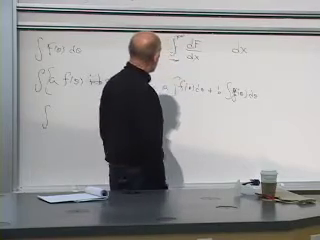
\includegraphics[width=0.88\textwidth]{lecture_06_figure_05.png}
\lectureframe{01:26:31.594}
\caption{這是貝雷津積分的普通原型：全導數的積分可化為端點值；若函數在端點趨近於零，積分便為零。黑板下方的推導有部分被遮住，因此正文列出了完整的方程。}
\end{figure}

我們希望格拉斯曼積分具有線性，並具備全導數積分為零這項實用性質。對單一奇座標，要求
\begin{align}
\int d\theta\,[af(\theta)+bg(\theta)]
&=
a\int d\theta\,f(\theta)
+b\int d\theta\,g(\theta),\\
\int d\theta\,\partial_\theta f(\theta)&=0.
\end{align}
第二個條件是測度平移不變性在代數上的類比。奇數座標軸沒有端點，也不會將它分割成微小區間後逐段求和。

\begin{classroomqa}
\audiencequestion{若沒有不定格拉斯曼積分，是否就得放棄「積分是微分的反運算」這個想法？\lecturetimestamp{01:21:19}}
\lecturerresponse{是的。貝雷津積分是一個定義好的線性泛函，不是求原函數的運算。對單一格拉斯曼變數而言，它實際上可由與微分相同的代數運算表示。}
\end{classroomqa}

\begin{classroomqa}
\audiencequestion{對整個時空的\(d^4x\)積分也是定積分嗎？\lecturetimestamp{01:21:34}}
\lecturerresponse{是的。對作用量在時空上積分時，邊界條件是默認的。兩者的差異在於，普通時空積分可以透過和的極限來理解；格拉斯曼積分則是以代數方式定義，其作用對象是有限基底\(1,\theta\)。}
\end{classroomqa}

\subsection{單一變數}

單一奇變數的任意函數，都可以寫成係數依固定次序置於右側的形式：
\begin{equation}
f(\theta)=a+\theta b.
\end{equation}
由於\(\partial_\theta\theta=1\)，全導數規則意味著
\begin{equation}
\int d\theta\,1=0.
\end{equation}
剩下的歸一化條件取為
\begin{equation}
\int d\theta\,\theta=1.
\end{equation}
因此，
\begin{equation}
\int d\theta\,f(\theta)=b.
\end{equation}
積分會選出最高次項的係數。在此採用左導數約定時，
\begin{equation}
\partial_\theta f=b
=\int d\theta\,f.
\end{equation}

\begin{classroomqa}
\audiencequestion{是否存在一個函數\(F(\theta)\)，使得\(\partial_\theta F=\theta\)？\lecturetimestamp{01:30:05}}
\lecturerresponse{不存在。這樣的函數必須含有一項與\(\theta^2\)成正比，但\(\theta^2=0\)。這也說明了為何格拉斯曼代數中沒有不定積分的類比。}
\end{classroomqa}

\subsection{兩個變數與測度的次序}

對一對複數變數\(\theta,\bar\theta\)，一般偶函數可寫成以下有序形式：
\begin{equation}
f(\theta,\bar\theta)
=a+\bar\theta\psi+\bar\psi\theta+b\,\bar\theta\theta.
\end{equation}
不會有更高次項，因為
\begin{equation}
\theta^2=\bar\theta^2=0,
\qquad
\bar\theta\theta=-\theta\bar\theta.
\end{equation}

現在固定以下約定：
\begin{equation}
\int d\theta\,d\bar\theta\,
\bar\theta\theta=1.
\end{equation}
在迭代積分中，相鄰的\(d\bar\theta\)積分先進行。於是得到下表：
\begin{align}
\int d\theta\,d\bar\theta\,1&=0,\\
\int d\theta\,d\bar\theta\,\theta&=0,\\
\int d\theta\,d\bar\theta\,\bar\theta&=0,\\
\int d\theta\,d\bar\theta\,\bar\theta\theta&=1.
\end{align}
因此，
\begin{equation}
\int d\theta\,d\bar\theta\,
f(\theta,\bar\theta)=b.
\end{equation}

\begin{classroomqa}
\audiencequestion{對於一個與\(\theta\)成正比的項，真的會是對\(\theta\)積分使二重積分歸零嗎？\lecturetimestamp{01:34:59}}
\lecturerresponse{不是；剛才的講解把兩者的作用顛倒了。先對\(\theta\)以\(\theta\)積分，結果為一。積分後的結果不再含有\(\bar\theta\)，而剩下對一的\(\bar\theta\)積分會歸零。無論如何，只有兩個變數都出現時，二重積分才不為零。}
\end{classroomqa}

\begin{classroomqa}
\audiencequestion{若將\(\theta\)與\(\bar\theta\)對調，積分會變號嗎？\lecturetimestamp{01:36:33}}
\lecturerresponse{會。奇變數與奇測度彼此反交換。依照上述約定，
\[
\int d\bar\theta\,d\theta\,\bar\theta\theta=-1.
\]
因此必須選定一種次序並始終一致。物理結果不受約定影響，但中間計算的符號會受影響。}
\end{classroomqa}

對於\(n\)個獨立的格拉斯曼變數，規則一目了然：
\begin{equation}
\int d\theta_n\cdots d\theta_1\,
f(\theta_1,\ldots,\theta_n)
\end{equation}
會取出有序最高次單項式\(\theta_1\cdots\theta_n\)的係數；符號則由所選的變數與測度次序決定。這項簡單的分量提取規則，是構造超空間作用量的關鍵。超對稱變分會成為奇全導數，而超空間積分會將其消去；這就如同普通作用量在適當邊界條件下會消去時空全導數。

\section{如此簡單的微積分為何有如此大的威力}

這些規則看起來幾乎微不足道：
\begin{equation}
\int d\theta\,1=0,
\qquad
\int d\theta\,\theta=1.
\end{equation}
然而，它們讓我們得以構造相互作用場論，並自動維持玻色子與費米子的質量及耦合之間的關係。超空間微積分的目的，與相對論中的張量微積分相同：安排記號，使所需的對稱性在每一項允許的運算下都能維持。

代價是必須仔細處理符號。每交換兩個奇物件，都會多出一個負號；因此，計算在概念上即使正確，也可能因一次次序選擇而出錯。這種困難並非表面問題，而是費米子統計在代數上的映現。

\begin{classroomqa}
\audiencequestion{格拉斯曼數是和超對稱一起發明的嗎？還是更早就已存在？\lecturetimestamp{01:41:19}}
\lecturerresponse{它們早已存在。赫爾曼・格拉斯曼在十九世紀發展出其背後的外代數。微分形式早已使用反交換的基底元素；到了二十世紀，量子場論與超對稱則為同一套數學找到了新的物理角色。}
\end{classroomqa}

現在可以開始進行具體構造了。超場收納完整的玻色子－費米子多重態，超空間導數維持代數結構，貝雷津積分則提取分量作用量。接下來，我們將先在最簡單的一維模型中運用這套方法，再將它應用於場論。
